
%{\bf Need some info about cosmic ray stand at Weizmann. }

With real detectors it will be possible to do more detailed
testing of the trigger processor. Testing with cosmic rays is an
important aspect of the trigger testing
plan. A cosmic ray test stand is not subject to test beam schedules,
allowing for rapid iteration and debugging in the early stages of
development. This is especially important because it allows both the
MM and sTGC systems to debug the interface with a real VMM chip.
Thus, part of the testing plan is to assemble realistic detector
prototypes for the MM and sTGC and place them in
cosmic ray telescopes.

It is important to ensure that
the cosmic ray muons used have sufficient momentum ($\mathcal{O}$\,(1\,GeV)) so as
to avoid the effects of multiple scattering. Additionally, it is useful
for the cosmic ray test setup to have a large angular acceptance, a
good angular resolution, and good timing resolution to allow precise
characterization of the trigger's behavior. Such test setups are
available at Harvard for the MM chambers and Weizmann for the sTGC
chambers. The test stands will include small-scale realistic detector setups,
including a small assembled MM octuplet and and two sTGC quadruplets.

The Harvard cosmic ray test setup consists of three planes of
scintillators sandwiching a 2\,m thick concrete block. It can detect
cosmic ray muons of greater than 0.8\,GeV with a time resolution better
than 1.5\,ns.  It has a coverage of 2.5\,m$^2$, an angular acceptance
of up to 25$^{\circ}$ from vertical and a 1.5$^{\circ}$ angular resolution.

The Weizmann test stand is designed to hold up to two 60\,cm $\times$ 40\,cm quadruplets.
A VMM configuration system was built to configure up to 12~chains of VMM chips.
There is one scintillator above and one below.
The lower scintillator has $\approx$20\,cm of lead shielding between it and the detectors to ensure that only hard cosmic muons are triggered.
The quadruplets were outfitted with VMM1 boards connected to strips and pads. (See Figure\,\ref{fig:WeizmannQuardupletCosmicSetup}.)
The VMM1 trigger outputs were connected via cables to the demonstrator boards mentioned in Section\,\ref{sec:sTGCpattern}.
A dual-VMM2 board was designed to replace the VMM1 boards, but work on it was halted when the trigger outputs of the VMM2 were found to be disabled.
This work will continue with VMM3.


\begin{figure}[h]
  \centering
  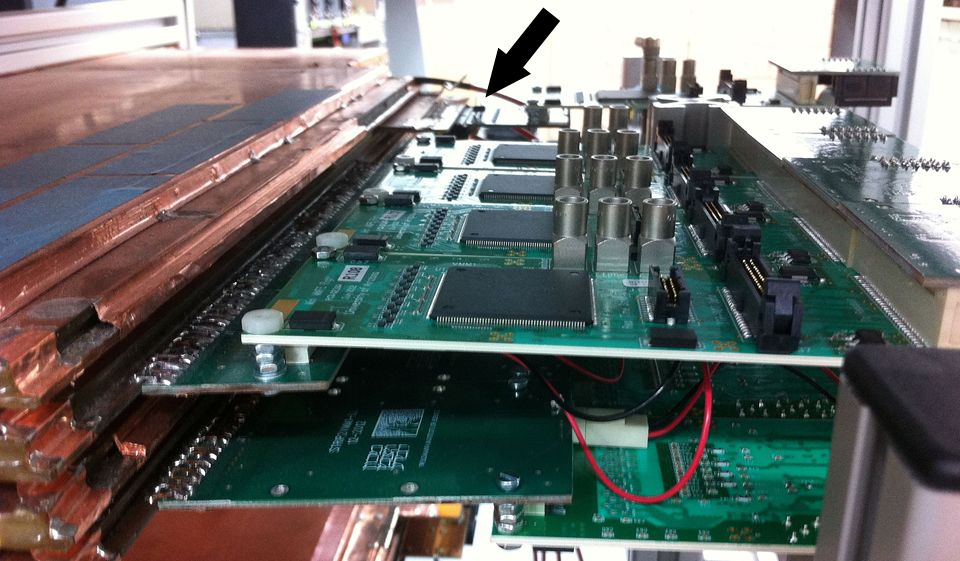
\includegraphics[width=0.85\textwidth]{figures/testing/WeizmannQuardupletCosmicSetup.JPG}
  \caption{sTGC quadruplet cosmic test setup. Shown a connection of two layers of a quadruplet. In each layer
  four VMM1 boards are connected to 64 strips and one VMM1 board (denoted by a black arrow) is connected to 16~pads.
  Other two layers of this quadruplet are connected on the opposite side.}
  \label{fig:WeizmannQuardupletCosmicSetup}
\end{figure}

\FloatBarrier

Once the realistic detector setups are assembled, the ultimate goal is to test the full
trigger chain with the chambers. First, the chain will be
tested with the trigger processor still in the evaluation board
platform, mainly testing the full communication pathway from chamber readout
to trigger processor. Once this is found to be working, the trigger
processor will move to its eventual home on the hardware platform in
an ATCA crate. There, more detailed tests with the cosmic rays can be
performed, including full measurements of the latency, trigger
efficiency, and hit throughput. Additionally, tests for the signal
integrity and bit errors through the whole electronics chain can be
done.

The key asset of the cosmic ray test setup is to be
able to iterate rapidly and debug issues that may arise without having
to wait for beam in a test beam setting.






